\documentclass[a4paper,10pt]{article}
\usepackage{fullpage}
\usepackage{times}
\usepackage{listings}
\usepackage{xparse}
\usepackage{hyperref}
\usepackage[a4paper, margin=1in]{geometry}

\usepackage{graphicx}
\graphicspath{ {./images/} }
\usepackage{subcaption}

%\usepackage{subfig}
\usepackage[
backend=biber,
style=ieee,
sorting=ynt
]{biblatex}


\addbibresource{references.bib}
 
\usepackage{xcolor}
 
\definecolor{codegreen}{rgb}{0,0.6,0}
\definecolor{codegray}{rgb}{0.5,0.5,0.5}
\definecolor{codepurple}{rgb}{0.58,0,0.82}
\definecolor{backcolour}{rgb}{0.95,0.95,0.92}
 
\lstdefinestyle{mystyle}{
    backgroundcolor=\color{backcolour},   
    commentstyle=\color{codegreen},
    keywordstyle=\color{magenta},
    numberstyle=\tiny\color{codegray},
    stringstyle=\color{codepurple},
    basicstyle=\ttfamily\footnotesize,
    breakatwhitespace=false,         
    breaklines=true,                 
    captionpos=b,                    
    keepspaces=true,                 
    numbers=left,                    
    numbersep=5pt,                  
    showspaces=false,                
    showstringspaces=false,
    showtabs=false,                  
    tabsize=2
}
 
\lstset{style=mystyle}
\NewDocumentCommand{\codeword}{v}{%
\texttt{{#1}}%
}


\iffalse
1. gather data from bb
2. run ./get_data.sh
3. run change clion deployment to remote
4. use jupyter locally
5. save everything
6. upload with ./upload_data_lib.sh
7. return to 1
\fi

\begin{document}

\title{L41: Lab 3 - The TCP State Machine, Latency, and Bandwidth}
\author{Nicolò Mazzucato \textless{}nm712\textgreater{}}
\date{\today}

\maketitle

\thispagestyle{empty}

\begin{abstract}           
   test
   - state machine comparison with the RFC[] one manually setting differnet latencies (differences on the final sequence)
   - analysis of the flow-control and congestion control mechanisms, plotting graphs with the congestion window, and analysing how the tcp state variable change in time.
   - behaviour of auto-resizing sockets buffer
   - the connection between Latency, RTT and bandwidth

\end{abstract}

\iffalse
- [0,5,10,20,40] ms available
General todos:
- (-s = not automatic, but set)
- [ ] write that the window advertisement is the space available in the receiver buffer.
- [ ] receive window comparison
- [ ] write that the cwnd is calculated on duplicate ACKs
- [ ] annotate trace with events from congestion control implementation
- [ ] packet loss detection (draw something red when a packet loss is detected)
- [ ] Mark when  the different tcp phases begin (slowstart, congestion avoidance, fast recovery?)
- [ ] compare flow-control and congestion limit, showing when each is limiting.
- [ ] understand if packet len is useful
- [ ] write about the dtrace buffer limitation
- [ ] Does linear increase in latency mean linear decrease in bandwidth? How does socket-buffer auto-resizing help/hurt/not change performance?
- [ ] Explore the effects of socket-buffer limits and stack graph information on the flow-control versus congestion-control limits. How does socket-buffer auto-resizing help/hurt/not change performance? 
- [ ] describe probe effect, if any?
- [ ] dtrace precision problem; There are many timestamps that are the same:v (put this in limitations)
- [ ] probe effect
\fi

\clearpage

\setcounter{page}{1}

\section{Introduction}


\section{Experimental setup and methodology}

\subsection{Hardware setup}

For the experiment, it is used the BeagleBone Black board with an open-source FreeBSD\cite{mckusick_design_2014} 11.0 operating system’s ARMv7 port. This board has the following characteristics:
\begin{itemize}
    \item 512MB DDR3 RAM
    \item 4GB 8-bit eMMC on-board flash storage
    \item AM335x 1GHz ARM® Cortex-A8 - Single core 32-bit processor\cite{noauthor_am3358_nodate}
    \begin{itemize}
        \item Independent 32KB L1 instructions and data cache
        \item Shared L2 cache (256KB)
        \item 64 bytes cache lines
    \end{itemize}
\end{itemize}

The board mounts an SD card. However, it is not relevant for the test, as the benchmark is in-memory.
      

\subsection {Methodology}

The benchmark consists of a program able to create two ends of a TCP socket over the loopback interface. The program is statically linked, so we can neglet dynamic linking performance overhead. The program opens a socket using the \codeword{socket(2)} system call, bind it to a specifc port, and listen for new connections. The receiving end similarly opens a socket, and uses \codeword{connect(2)} to connect with the other endpoint at the same port. During the benchmark, a fixed size amount of data is transferred from the sender to the receiver. Afterwards, the \codeword{close(2)} system call initiate the closing phase.

IPFW, the firewall used, provides DUMMYNET\cite{luigirizzo_luigirizzodummynet_2020}, that allows to shape the traffic. In this experiment, IPFW is used to generate two pipes, and sent the latency in each one of those. The pipes are used to filter the traffic, and selectively apply the delay only to the traffic we care abot. We then generate the state transition graph at different levels of delays, to see the differences.
The actors of the communication, in our case, are two threads: one that sends data, and the other that receives it. The dimension of the buffer passed to the \codeword{write(2)} system call are 128KB for the state-machine generation, and 1MB for the remaining graphs.
The total amount of data transferred is 16MB for each benchmark run.

The loopback Maximum Transmission Unit (MTU) is manually set to 1,500 bytes before each test. In this it is possible avoid larger values that might have been caused to the local nature of the test, resembling real LAN or WAN results.

DTrace is used for most performance measurements. In particualar, we use the following providers:

\begin{itemize}
   \item Function Boundary Tracing (FBT) provider. We are using probes on specific functions. There are also TCP generic ones, portable across different systems, but they do not provide the needed number of parameters to make all the analysis. The output from the tracing of the entire kernel's function is then visualized in Perfetto\cite{noauthor_perfetto_nodate}, to graphically inspect for futher interesting behaviours.
   \item Profile provider. It fires a probe at a given frequency. We use it to aggregate the results of \codeword{stack()}, and see where most of the time is spent. 
\end{itemize}

After each benchmark run, two seconds have been added before stopping the DTrace instumentation, to make sure to capture any final timing related event. Without those, the state transition graphs were sometimes different: often the time-wait phase was not reached, because it was entered after the benchmark end, when the DTrace instrumentation was not running anymore.

The verbose benchmark output, containing the IPC loop duration measured from the program, is then used to evaluate the probe-effect caused by DTrace.


All the benchmark runs are executed 11 times for each parameter value, and the first one is dropped. In each graph, it is possible to see the error as a vertical line. However, in almost all cases, this error is negligible, highlighting a controlled benchmarking environment. The main value on the graph is the median of the 10 measurements.



\subsection{Limitations}

During the tracing, several other processes were running, and this might have influenced the results. In particular:
\begin{itemize}
    \item One ssh session
    \item A Jupyter notebook
\end{itemize}



\section{Results and discussion}

\subsection{TCP state-transition diagram}
% todo insert diagram image and RFC image
%overall figure
\begin{figure}[]
\begin{subfigure}{.25\textwidth}
    \centering
    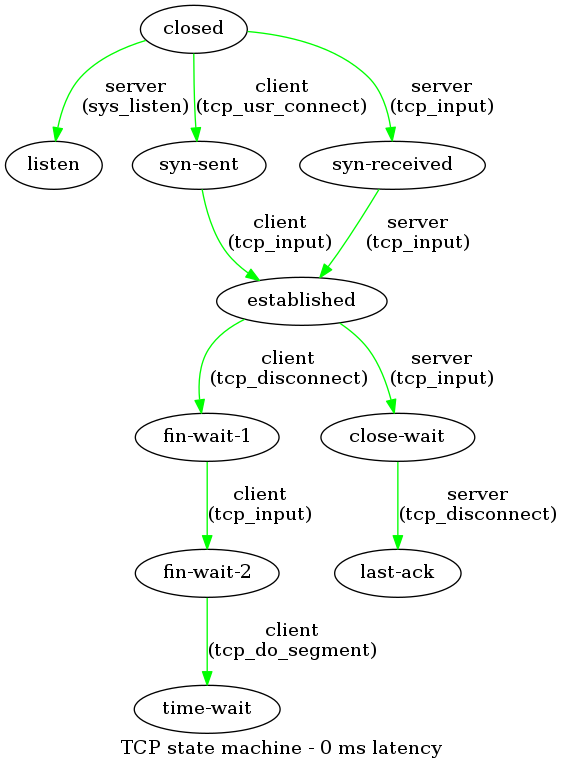
\includegraphics[width=\textwidth]{images/TCP_state_machine_0_ms.png}
    \caption{TCP state transition graph with 0ms latency.}
    \label{fig:0ms_latency}
\end{subfigure}%
\qquad
\begin{subfigure}{.25\textwidth}
   \centering
   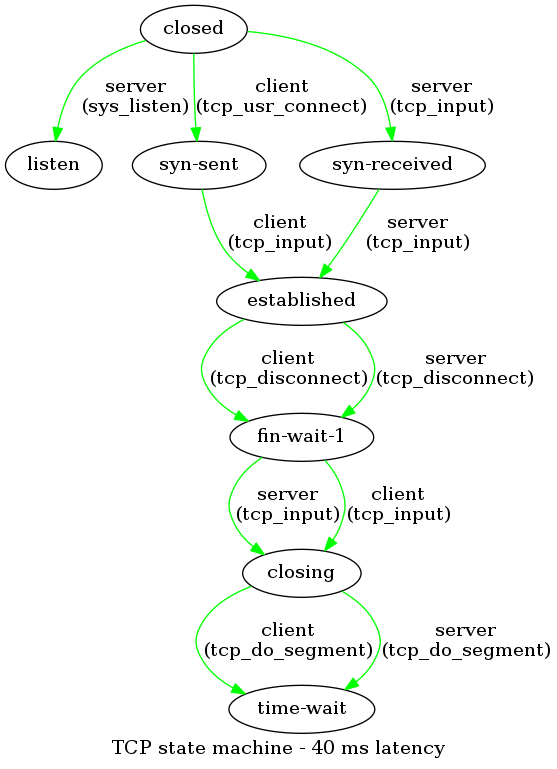
\includegraphics[width=\textwidth]{images/TCP_state_machine_40_ms.png}
    \caption{TCP state transition graph with 40ms latency.}
    \label{fig:40ms_latency}
\end{subfigure}
\qquad
\begin{subfigure}{.25\textwidth}
   \centering
   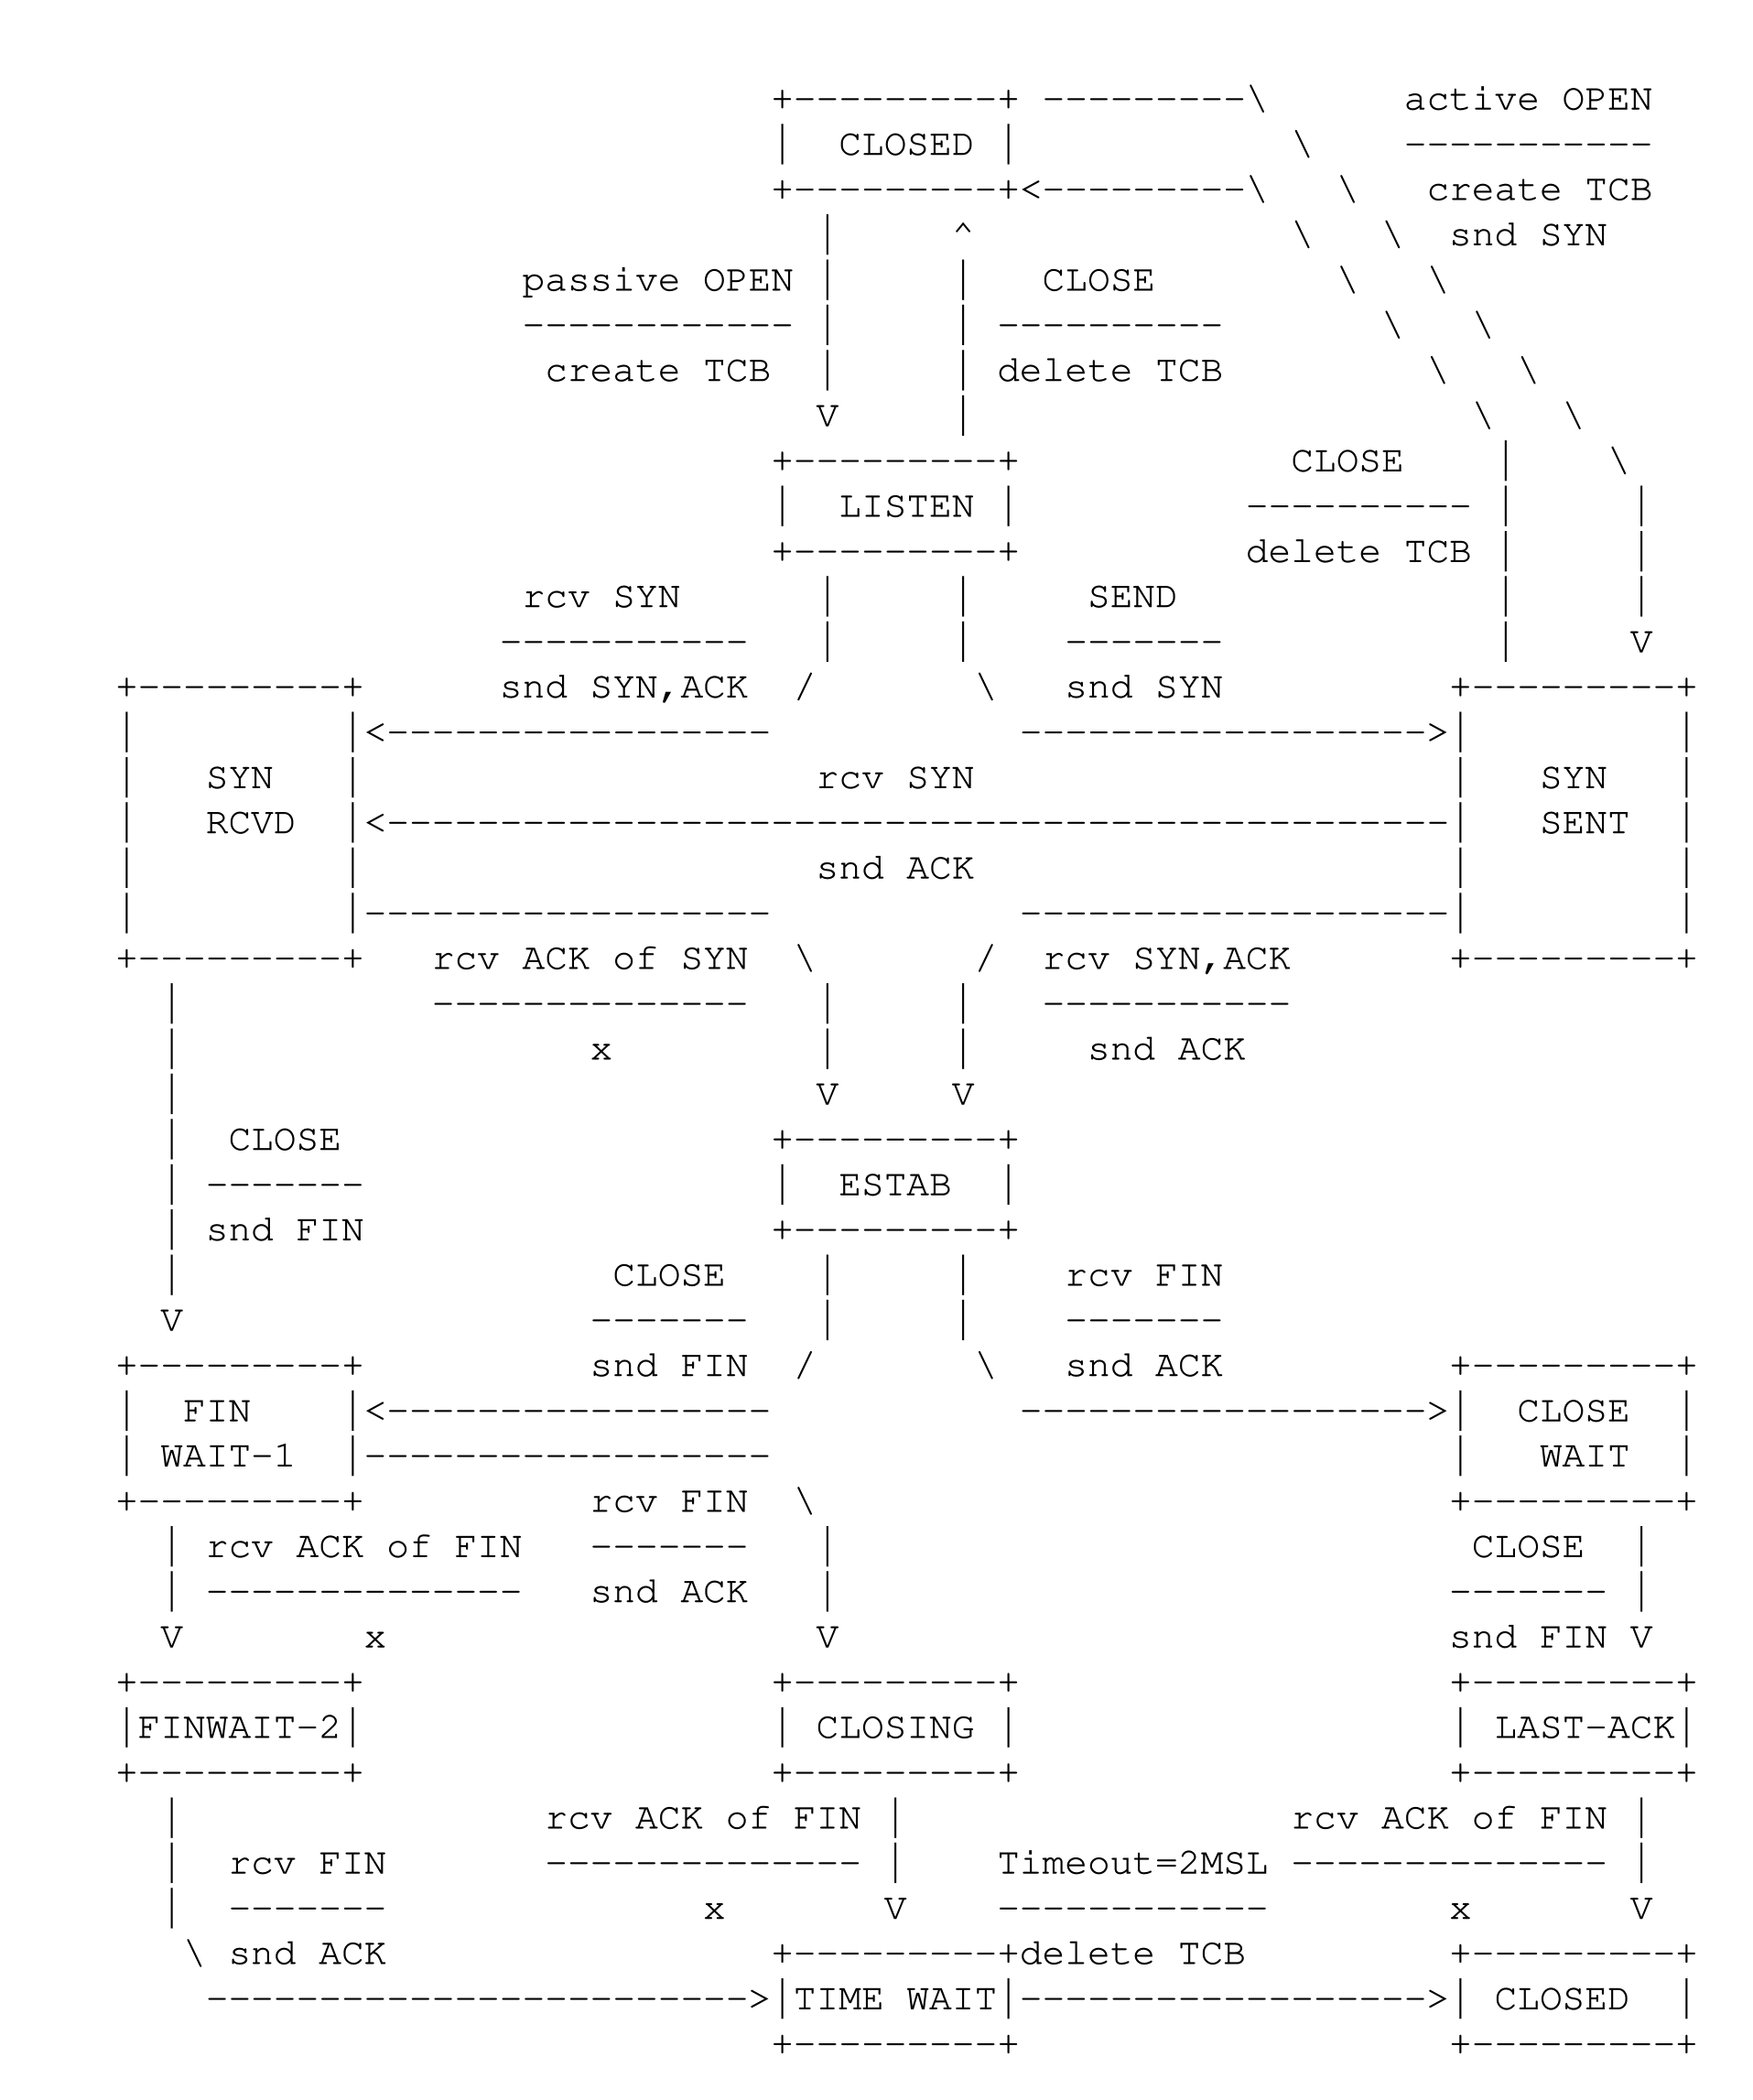
\includegraphics[width=\textwidth]{images/RFC_Graph.png}
    \caption{TCP state transition according to RFC 793.}
    \label{fig:RFC_graph}
\end{subfigure}
\caption[short]{Comparison between measured state transitions and RFC 793.}
\end{figure}

We generated TCP state transition graphs with different latency values, from 0ms to 40ms, with 5ms steps. It is possible to notice that from a latency value of 10ms there is a slighly different shape in the connection closing phase. In particular:
\begin{itemize}
   \item With 0 ms latency, as shown in figure \ref{fig:0ms_latency}, the close phase of the connection goes through the \codeword{fin-wait-1} and \codeword{fin-wait-2} states (client side)
   \item From a latency of 10ms onwards, as shown in figure \ref{fig:40ms_latency}, both the server and the client reach the \codeword{fin-wait-1} state, but then they both enter into the closing state, without passing through the \codeword{fin-wait-2} state.
\end{itemize}

This behaviour is clearly explained in the RFC 793\cite{postel_transmission_nodate} at page 42. In the former case, it happens that the server sends the close packet (with the \codeword{FIN}), then the client receives it before closing the connection itself.
In the latter case we have that due to the delay, the connection is closed simultaneously by both actors. None of them will receive the other FIN before sending its own FIN. For this reason, they both switch to fin-wait-1. When they receive each other FIN, they switch to closing, and after having received the ACK of the FIN, they go to the time-wait state.

There is another small difference between the generated graph and the RFC one. The server, does not transition from listen to \codeword{syn-received}, but from closed to \codeword{syn-receive}. In the RFC graph there are other transitions not performed during the benchmark, related to cases such as the closing of a connection before the proper enstablishment.

% todo probe effect? in this case not relevant I think, but how to mseasure it? probably overall time at each delay level?


\subsection{Bandwidth for each imposed latency}

\begin{figure}[h]
\centering
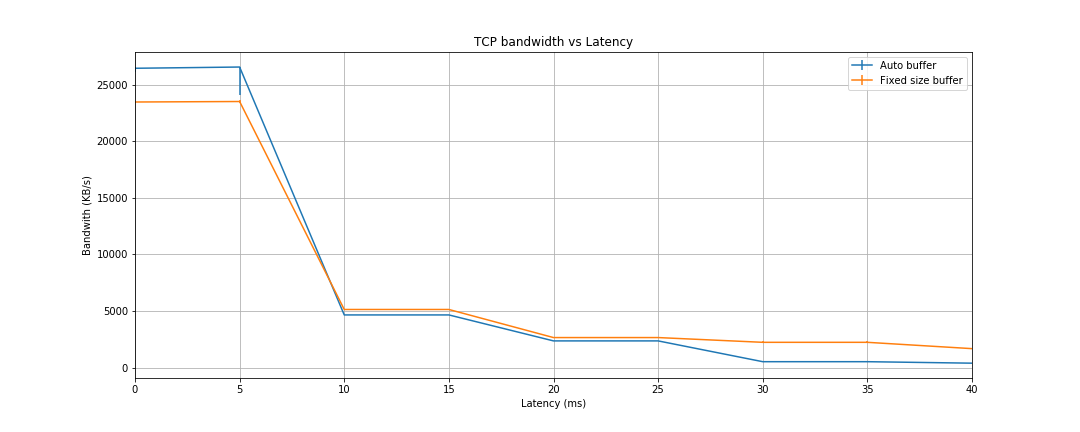
\includegraphics[width=\textwidth]{images/tcp_bandwidth.png}
  \caption{Imposed DUMMYNET lantecy vs bandwidth, both with and without socket-buffer auto-resizing}
   \label{fig:bandwidth}
\end{figure}

Figure \ref{fig:bandwidth} shows the bandwidth versus the DUMMYNET-imposed latency. We can notice that the bandwidth decrease is not linear. It remains almost constant until a latency of 5ms, when if suddently drops at 10ms. At 20ms, it halves again, to then stay stationary from 30ms onwards.
The socket-buffer autoresizing does not always result in a performance increase. We can notice two phases:
\begin{itemize}
   \item With low latencies, until 5ms, the auto-resizing policy allows an higher bandwidth.
   \item From 10ms to 25ms, the benchmark without autoresizing is always slighly faster than the statically sized one, but comparable.
   \item From 30ms onwards the statically sized one allows a bandwidth more than double the autosized one. %todo find the reson!
\end{itemize}

There can be multiple reason for this trend. An increased latency limits the congestion window grow, and as a consequence the overall bandwidth, because the "final" transfer rate will be reached more slowly.
% todo write more here!

\subsection{Time-bandwidth graph}

\iffalse 
Notes:
- with manual socket it seems faster: it finishes in 2.7 instead of 3.4
- for the congestion window, initial values are trimmed out
\fi

\subsection{Probe effect}

\section{Conclusions}

Some conclusions
\newpage

\section{References}

\printbibliography

\section{Appendices}


\end{document}
